\documentclass[12pt] {article}

%%% Preambuła %%%
\usepackage[T1]{fontenc}
\usepackage[polish]{babel}
\usepackage[utf8]{inputenc}
\usepackage{lmodern}
\usepackage{hyperref}
\usepackage{mathptmx}
\usepackage{float}
\usepackage{graphicx}
\usepackage{amsmath}
\usepackage{xcolor}
\usepackage{listings}
\selectlanguage{polish}

\usepackage{geometry}

\geometry{
 a4paper,
 total={170mm,257mm},
 left=20mm,
 top=20mm,
 }


\usepackage{forest}

\definecolor{folderbg}{RGB}{124,166,198}
\definecolor{folderborder}{RGB}{110,144,169}

\def\Size{4pt}
\tikzset{
      folder/.pic={
        \filldraw[draw=folderborder,top color=folderbg!50,bottom color=folderbg]
          (-1.05*\Size,0.2\Size+5pt) rectangle ++(.75*\Size,-0.2\Size-5pt);  
        \filldraw[draw=folderborder,top color=folderbg!50,bottom color=folderbg]
          (-1.15*\Size,-\Size) rectangle (1.15*\Size,\Size);
      }
    }

%%% Ustawienia listingów %%%
\definecolor{vgreen}{RGB}{104,180,104}
\definecolor{vblue}{RGB}{49,49,255}
\definecolor{vorange}{RGB}{255,143,102}

\lstdefinestyle{verilog-style}
{
    language=Verilog,
    basicstyle=\small\ttfamily,
    keywordstyle=\color{vblue},
    identifierstyle=\color{black},
    commentstyle=\color{vgreen},
	frame=single,
    tabsize=8,
    moredelim=*[s][\colorIndex]{[}{]},
    literate=*{:}{:}1
}

\makeatletter
\newcommand*\@lbracket{[}
\newcommand*\@rbracket{]}
\newcommand*\@colon{:}
\newcommand*\colorIndex{%
    \edef\@temp{\the\lst@token}%
    \ifx\@temp\@lbracket \color{black}%
    \else\ifx\@temp\@rbracket \color{black}%
    \else\ifx\@temp\@colon \color{black}%
    \else \color{vorange}%
    \fi\fi\fi
}
\makeatother


%%% Strona tytułowa %%%
\title {
	Języki Opisu Sprzętu \\
	\large Projekt: Elektroniczny Sejf Hotelowy \\
	Dokumentacja}

\author {
	Arkadiusz Kasprzak \\
	Jarosław Cierpich \\
	Wydział Fizyki i Informatyki Stosowanej \\ 
	Informatyka Stosowana}

	
\begin{document}

\begin{figure}
\centering

\includegraphics[scale = 1.5]{res/agh_znk_wbr_cmyk}
\end{figure}

%%% Strona tytułowa %%%
\maketitle

%%% Spis treści %%%
\newpage
\tableofcontents

\newpage
\section{Wstęp}
Niniejszy dokument stanowi dokumentację projektu \textbf{Elektroniczny Sejf Hotelowy} wykonanego w ramach przedmiotu \textbf{Języki Opisu Sprzętu} (WFiIS AGH) przez Jarosława Cierpicha i Arkadiusza Kasprzaka. Dokument ten zawiera m.in. założenia projektowe oraz opis wymaganej funkcjonalności, dokumentację przeznaczoną dla użytkownika projektu, dokumentację techniczną, analizę procesu syntezy oraz opis procedury testowania.

\section{Projekt}
Ten rozdział poświęcony został opisowi założeń projektowych oraz wymaganej funkcjonalności.

\subsection{Założenia projektowe}
Projekt dostarczać ma funkcji elektronicznego sejfu hotelowego, to znaczy pozwalać ma na otwieranie go za pomocą z góry ustalonego szyfru oraz późniejsze zamknięcie go. Projekt ma być zrealizowany na płytce rozwojowej \textbf{Zedboard} (do Xilinx Zynq-7000). Ze względu na okoliczności wykonywania projektu (projekt jako zaliczenie przedmiotu) przyjęte zostały pewne uproszczenia:
\begin{itemize}
\item czujnik zamknięcia sejfu zastąpiony zostaje przełącznikiem obsługiwanym przez użytkownika
\item szyfr jest parametrem projektu - nie jest możliwa jego modyfikacja na płytce bez powtórzenia procesu syntezy i implementacji
\item ruch rygla reprezentowany jest za pomocą dwóch diod LED dostępnych na płytce
\end{itemize}
Do realizacji projektu użyty ma być język \textbf{SystemVerilog} oraz środowisko \textbf{Xilinx Vivado}. 
Szyfr składać ma się z trzech liczb z przedziału \lbrack 0; 32). Liczby mają być wprowadzane przez użytkownika za pomocą pokrętła, przy czym kierunek obrotu pokrętła wskazuje, która liczba jest aktualnie wprowadzana: ruch zgody ze wskazówkami zegara oznacza pierwszą lub trzecią liczbę, ruch przeciwny do wskazówek zegara - drugą liczbę. Wprowadzenie nieprawidłowej liczby ma przerywać proces podawania szyfru - tzn. układ nie czeka, aż wprowadzony zostanie cały szyfr. Aktualnie wprowadzona liczba ma być prezentowana za pomocą wyświetlacza OLED.
Układ ma być w miarę możliwości pozbawiony błędów związanych z drganiami styków czy niestandardowym działaniem użytkownika.

\subsection{Wymagana funkcjonalność}
Od projektu wymaga się dostarczenia następującej funkcjonalności:
\begin{itemize}
\item możliwość wprowadzenia przez użytkownika poprawnego szyfru składającego się z trzech liczb z zakresu \lbrack 0; 32) za pomocą pokrętła
\item możliwość wprowadzenia przez użytkownika niepoprawnego szyfru, co automatycznie przerwać ma proces otwierania sejfu
\item możliwość monitorowania przez użytkownika aktualnego stanu otwarcia sejfu - za pomocą diod LED
\item możliwość monitorowania przez użytkownika aktualnie wprowadzanej wartości - za pomocą wyświetlacza OLED
\item możliwość rozpoczęcia procesu otwierania sejfu - za pomocą przycisku \textit{Open}
\item możliwość zamknięcia sejfu - za pomocą przycisku \textit{Close}
\item możliwość ustalenia aktualnej pozycji rygla sejfu - za pomocą przełącznika - zastępuje to czujnik zamknięcia sejfu
\item możliwość łatwego zaprogramowania nowego szyfru - zmiana trzech wartości w kodzie 
\end{itemize}




\section{Dokumentacja użytkownika}




\section{Dokumentacja techniczna}

\subsection{Warstwa Hardware}

\subsection{Warstwa Software - architektura}
Poniższy diagram przedstawia wysokopoziomową architekturę projektu:\\
\textbf{TUTAJ DAC DIAGRAM}\\
Poniższy diagram przedstawia strukturę modułów i połączeń między nimi zastosowaną w projekcie:\\
\textbf{TUTAJ DAC DIAGRAM}\\
Wysokopoziomowa struktura katalogów i plików przedstawiona została poniżej:\\
\begin{forest}
      for tree={
        font=\ttfamily,
        grow'=0,
        child anchor=west,
        parent anchor=south,
        anchor=west,
        calign=first,
        inner xsep=7pt,
        edge path={
          \noexpand\path [draw, \forestoption{edge}]
          (!u.south west) +(7.5pt,0) |- (.child anchor) pic {folder} \forestoption{edge label};
        },
        % style for your file node 
        file/.style={edge path={\noexpand\path [draw, \forestoption{edge}]
          (!u.south west) +(7.5pt,0) |- (.child anchor) \forestoption{edge label};},
          inner xsep=2pt,font=\small\ttfamily
                     },
        before typesetting nodes={
          if n=1
            {insert before={[,phantom]}}
            {}
        },
        fit=band,
        before computing xy={l=15pt},
      }  
		[TopSafe
			[TopSafe.xpr,file]
			[TopSafe.srcs
				[constrs\_1]
				[sim\_1]
				[sources\_1]
      		]
      	]	
\end{forest} \\
Struktura wewnętrzna katalogu \textbf{constrs\_1} jest następująca: \\ 
\begin{forest}
      for tree={
        font=\ttfamily,
        grow'=0,
        child anchor=west,
        parent anchor=south,
        anchor=west,
        calign=first,
        inner xsep=7pt,
        edge path={
          \noexpand\path [draw, \forestoption{edge}]
          (!u.south west) +(7.5pt,0) |- (.child anchor) pic {folder} \forestoption{edge label};
        },
        % style for your file node 
        file/.style={edge path={\noexpand\path [draw, \forestoption{edge}]
          (!u.south west) +(7.5pt,0) |- (.child anchor) \forestoption{edge label};},
          inner xsep=2pt,font=\small\ttfamily
                     },
        before typesetting nodes={
          if n=1
            {insert before={[,phantom]}}
            {}
        },
        fit=band,
        before computing xy={l=15pt},
      }  
		[constrs\_1
			[new
				[constraints.xdc,file]
      		]
      	]	
\end{forest} \\
Struktura katalogu zawierającego moduły testowe: \\
\begin{forest}
      for tree={
        font=\ttfamily,
        grow'=0,
        child anchor=west,
        parent anchor=south,
        anchor=west,
        calign=first,
        inner xsep=7pt,
        edge path={
          \noexpand\path [draw, \forestoption{edge}]
          (!u.south west) +(7.5pt,0) |- (.child anchor) pic {folder} \forestoption{edge label};
        },
        % style for your file node 
        file/.style={edge path={\noexpand\path [draw, \forestoption{edge}]
          (!u.south west) +(7.5pt,0) |- (.child anchor) \forestoption{edge label};},
          inner xsep=2pt,font=\small\ttfamily
                     },
        before typesetting nodes={
          if n=1
            {insert before={[,phantom]}}
            {}
        },
        fit=band,
        before computing xy={l=15pt},
      }  
		[sim\_1
      		[new
      			[OLED
      				[TbOledDriver.sv,file]
      			]
				[TbBcd2Decades.sv,file]
				[TbClkDiv.sv,file]
				[TbDebouncerButtons.sv,file]
				[TbDelay.sv,file]
				[TbDigitCompare.sv,file]
				[TbLedDriver.sv,file]
				[TbMasterFsm.sv,file]
				[TbRseDecoder.v,file]
				[TbSafeTop.sv,file]
			]
		]
\end{forest} \\
Struktura katalogu zawierającego kod źródłowy projektu: \\		
\begin{forest}
      for tree={
        font=\ttfamily,
        grow'=0,
        child anchor=west,
        parent anchor=south,
        anchor=west,
        calign=first,
        inner xsep=7pt,
        edge path={
          \noexpand\path [draw, \forestoption{edge}]
          (!u.south west) +(7.5pt,0) |- (.child anchor) pic {folder} \forestoption{edge label};
        },
        % style for your file node 
        file/.style={edge path={\noexpand\path [draw, \forestoption{edge}]
          (!u.south west) +(7.5pt,0) |- (.child anchor) \forestoption{edge label};},
          inner xsep=2pt,font=\small\ttfamily
                     },
        before typesetting nodes={
          if n=1
            {insert before={[,phantom]}}
            {}
        },
        fit=band,
        before computing xy={l=15pt},
      }  
		[sources\_1
			[new
				[Bcd2Decades.sv,file]
				[ClockDiv.sv,file]
				[DebouncerButtons.sv,file]
				[DebouncerKnob.v,file]
				[DigitCompare.sv,file]
				[LedDriver.sv,file]
				[MasterFsm.sv,file]
				[safeTop.sv,file]
				[RseDecoder.sv,file]
				[OLED
					[delay.sv,file]
					[fsm\_init.sv,file]
					[fsm\_oper.sv,file]
					[OledDriver.sv,file]
					[pixel\_SSD1306.dat,file]
					[rom.v,file]
					[screens.vh,file]
					[spi.sv,file]
					[update\_page.sv,file]
				]	
			]
		]
\end{forest}


\subsection{Warstwa Software - parametry i moduły projektu}
Ten podrozdział opisuje część implementacji projektu - zastosowane parametry oraz moduły napisane w języku SystemVerilog.

\subsubsection{Parametry projektu}
Główny moduł projektu udostępnia następujące \textbf{parametry} pozwalające na modyfikację działania sejfu:
\begin{itemize}
\item \textit{slowClockPeriodLength} - współczynnik oznaczający wartość dzielnika częstotliwości zegara, którym taktowany jest sejf (z wyjątkiem debouncerów i wyświetlacza OLED). Wartość domyślna: 100000.
\item \textit{debouncerClockPeriodLength} - współczynnik oznaczający wartość dzielnika częstotliwości zegara, którym taktowane są debouncery w projekcie. Wartość domyślna: 300007.
\item \textit{areDebouncersUsed} - flaga włączająca lub wyłączająca generację debouncerów w projekcie. Wartość domyślna: 1 - debouncery mają zostać wygenerowane.
\item \textit{firstCodeNumber} - pierwsza liczba szyfru. Wartość domyślna: 15.
\item \textit{secondCodeNumber} - druga liczba szyfru. Wartość domyślna: 30.
\item \textit{thirdCodeNumber} - trzecia liczba szyfru. Wartość domyślna: 9.
\end{itemize}

\subsubsection{Moduły projektu}
Projekt składa się z następujących \textbf{modułów}:
\begin{itemize}
\item SafeTop - główny moduł projektu
\item Bcd2Decades - licznik BCD (Binary Coded Decimal) o dwóch dekadach
\item ClockDiv - dzielnik zegara
\item DebouncerButtons - układ wygaszający drgania na przyciskach
\item DebouncerKnob - układ wygaszający drgania na pokrętle
\item DigitCompare - układ porównujący wprowadzone przez użytkownika liczby z szyfrem 
\item LedDriver - sterownik diod LED
\item MasterFsm - główna logika sejfu
\item RseDecoder - układ odpowiedzialny za komunikację z pokrętłem
\item Moduły odpowiedzialne za obsługę wyświetlacza OLED: 
\begin{itemize}
\item OledDriver
\item delay
\item fsm\_init
\item fsm\_oper
\item rom
\item spi
\item update\_page
\end{itemize}
\end{itemize}
Ponadto projekt zawiera \textbf{dwa inne pliki} związane z obsługą wyświetlacza OLED:
\begin{itemize}
\item screens.vh
\item pixel\_SSD1306.dat
\end{itemize}
W dalszej części zaprezentowane zostanie działanie poszczególnych modułów.

\paragraph{SafeTop}

\section{Analiza procesu syntezy}

\section{Testy}
Ostatni rozdział poświęcony został procesowi testowania projektu - w tym przygotowanym modułom testowym oraz procesowi testowania manualnego. 

\subsection{Moduły testujące}
Projekt zawiera \textbf{TUTAJ WSTAWIC ILE} modułów testowych (tzw. moduły \textit{Testbench}). Umożliwiają one przeprowadzenie symulacji działania modułów projektu. Moduły testowane były za pomocą dwóch typów symulacji:
\begin{itemize}
\item symulacja behawioralna (\textit{behavioral simulation})
\item symulacja po syntezie z uwzględnieniem parametrów czasowych (\textit{post-synthesis timing simulation})
\end{itemize}
\textbf{TUTAJ WSTAWIC STRUKTURE TB}
Podstawowa struktura większości modułów \textit{Testbench} jest podobna - składają się one z:
\begin{itemize}
\item deklaracji parametrów wejściowych modułu (jeśli takie są)
\item deklaracji zmiennych stanowiących wejścia i wyjścia testowanego modułu oraz zmiennej odpowiadającej za \textit{Global System Reset - GSR}
\item instancji testowanego modułu (\textit{UUT - Unit Under Test})
\item generacji sygnałów wejściowych testowanego modułu (w tym zwykle sygnału zegara i resetu)
\end{itemize}
Listing \ref{lst:testy} ilustruje opisaną powyżej strukturę.

\begin{lstlisting}[style={verilog-style}, caption={Uproszczona struktura wykonanych modułów testujących}, label={lst:testy}]
module TbExample();
    
    // parametry    
    localparam mod = 3;    
    
    // wejscia
    reg clk, rst;
    reg in1;
    
    // wyjscia
    reg [3:0] out1; 
    
    // ...

    // GSR - Global System Reset
    wire gsr = glbl.GSR;

    // UUT - Unit Under Test
    ExampleModule #(.mod(mod)) EXAMPLE (
        .clk(clk), .rst(rst), .in1(in1), .out1(out1));

    // generacja sygnalow wejsciowych

    // zegar
    initial begin
        clk = 1'b0;
        @(negedge gsr);
        forever #5 clk = ~clk;
    end
    
    // reset
    initial begin
        rst = 1'b1;
        @(negedge gsr);
        #5 rst = 1'b0;
    end
    
    // in1
    initial begin 
        // kod generujacy wartosci sygnalu in1
    end
    
    // ...
    
endmodule
\end{lstlisting}

W dalszej części tego podrozdziału omówione zostaną poszczególne moduły testujące oraz wyniki przeprowadzonych symulacji behawioralnych. 

\subsubsection{Testy modułu Bcd2Dec}


\begin{figure}[H]
\centering
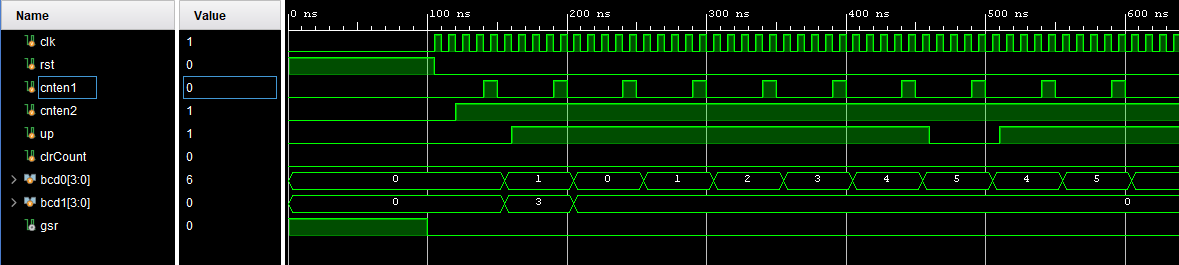
\includegraphics[width=\textwidth]{res/behav_sims/Bcd2Dec_behavSim_1.png}
\caption{Tutaj dac opis}
\end{figure}

\begin{figure}[H]
\centering
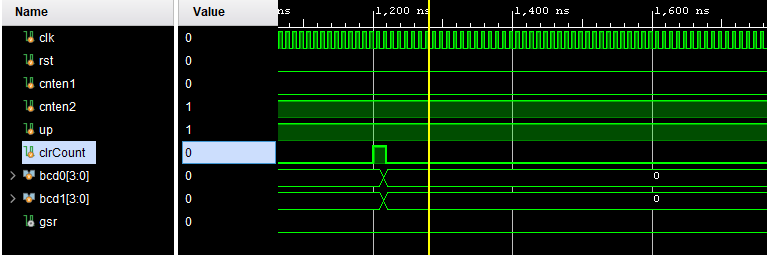
\includegraphics[width=\textwidth]{res/behav_sims/Bcd2Dec_behavSim_2.png}
\caption{Tutaj dac opis}
\end{figure}


\subsubsection{Testy modułu ClkDiv}

\subsection{Testy manualne}



\end{document}